\chapter{電磁界解析}

\section{電磁界シュミレータ}
本研究では以下に示す電磁界解析シュミレーターを用いて空洞共振器の設計を行った。
使用したシュミレーターはMW-Studio(CST社)\cite{CST}であり、
以下の2つの解析モードを用いた\cite{MWS-1}。

\subsection*{固有値解析}
固有値解析モードでは、共振器の構造や材質から、共振器内の電磁場分布をMaxwell方程式の固有値解析から求める。
様々な共振周波数に対応する電磁場の空間分布を把握する事ができる。
本研究では、共振器に誘電体を挿入したり、同軸ケーブルを挿入した場合の、
共振モードとその電磁場分布、共振周波数を知るために使用した。

\subsection*{過渡解析(トランジェント解析)}
過渡解析(トランジェント解析とも言う)モードでは、
共振器内にマイクロ波パルスを入力し、
その応答をフーリエ変換して周波数特性を解析する。
共振器の透過特性の解析には、
マイクロ波を入射するためのポートと透過波を取り出すポートを設定する必要がある。
過渡解析モードは、共振器と外部伝送路の結合条件を解析するために用いる。

\subsection*{有限積分法}
MW-StudioはFIT(有限積分法)が用いられている
\cite{MWS-2}。
FITは普遍的な空間離散化スキームをもたらす数値解析手法であり、
T.Weilandにより初めて提唱された\cite{FIT}。
FITは他の多くの数値解析手法のような微分形式ではなく、
以下のような積分形式のマクスウェル方程式を離散化して計算を行う。

\begin{eqnarray}
  \oint_{\partial A} \mathbf{E} \cdot d\mathbf{s}
  = - \int_{\partial A} \frac{\partial \mathbf{B}}{\partial t} \cdot d  \mathbf{A}\\
  \oint_{\partial A} \mathbf{H} \cdot d\mathbf{s} =  \int_{\partial A} \{ \frac{\partial \mathbf{D}}{\partial t} + \mathbf{J} \} \\
  \oint_{\partial V} \mathbf{D} \cdot d\mathbf{A} = \int_V \rho dV \\
  \oint_{\partial V} \mathbf{B} \cdot d\mathbf{A} = 0
\end{eqnarray}

これらの方程式を解く際には、解析対象を包含するような
有限の計算領域を定義する必要がある。
この領域を適切なメッシュシステムを用いて複数個の小さなグリッドセルに分割する。

\vspace{10 mm}

\begin{figure}[h]
  \begin{center}
    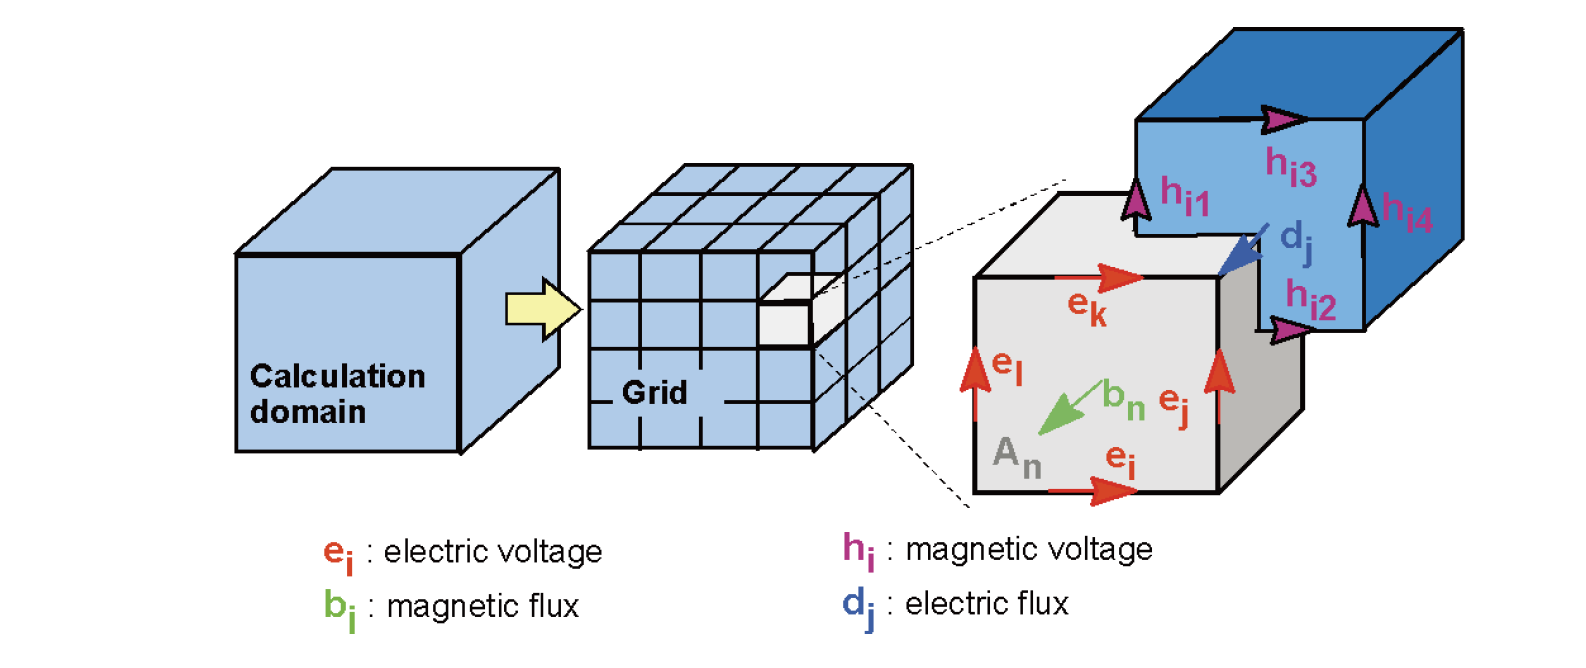
\includegraphics[width=12cm]{./image/mesh.png}
    \caption{メッシュへの分割\cite{MWS-2}}
    \label{fig:Mesh}
  \end{center}
\end{figure}

このグリッドセルごとにマクスウェル方程式を解くことを繰り返すと、
全体の計算をある行列形式で表すことができる。
これにより、FIT法は一般的の有限要素法に比べ、
メッシュ数の増大に伴う計算時間の増加がはるかに小さい。
% つまり、このメッシュの数が計算精度に大きく関わり、
% メッシュ数をあげればあげるほど精度は高くなるが、計算時間も長くなっていく。
しかしながら。過去の計算結果から、
メッシュ数を細かくしても微細加工をした
超伝導素子を置いた時の応答を調べることはできず、
実際に製作した場合と全く同じ条件でシミュレートすることはできないため、
実験とのずれは承知の上でシミュレーションを行った。
実際、メッシュ数が2000程度の場合、共振周波数の理論値と数値計算結果とのズレは1GHz以下であった。

\section{シミュレーションの基本設定}
シミュレーションの基本設定を以下に示す。

\begin{itemize}
  \item メッシュ数: 20000前後
  \item 空洞を構成する素材: 完全導体
  \item 周波数範囲: 30 〜 80GHz
  \item Accuracy: -40dB
\end{itemize}
% \begin{description}
%   \item[メッシュ数:] 20000前後
%   \item[空洞を構成する素材:] 完全導体(PEC)
%   \item[周波数範囲:] 30 〜 80GHz
%   \item[Accuracy:] -40dB
% \end{description}

ここでAccuracyとは、
解析空間内の電磁界エネルギーの総量が設定値まで減衰したら
計算を終了させるための設定値である。
また、解析する周波数範囲によりシミュレーションする周波数の刻みが変わり、
解析周波数範囲が大きいほど刻みも大きくなり、
解析周波数範囲が小さいと刻みも小さくなる。
